\subsection{The cross section of $K^0$}
\begin{figure}
  \centering
  \begin{tabular}{cc}
    \begin{minipage}{0.6\hsize}
      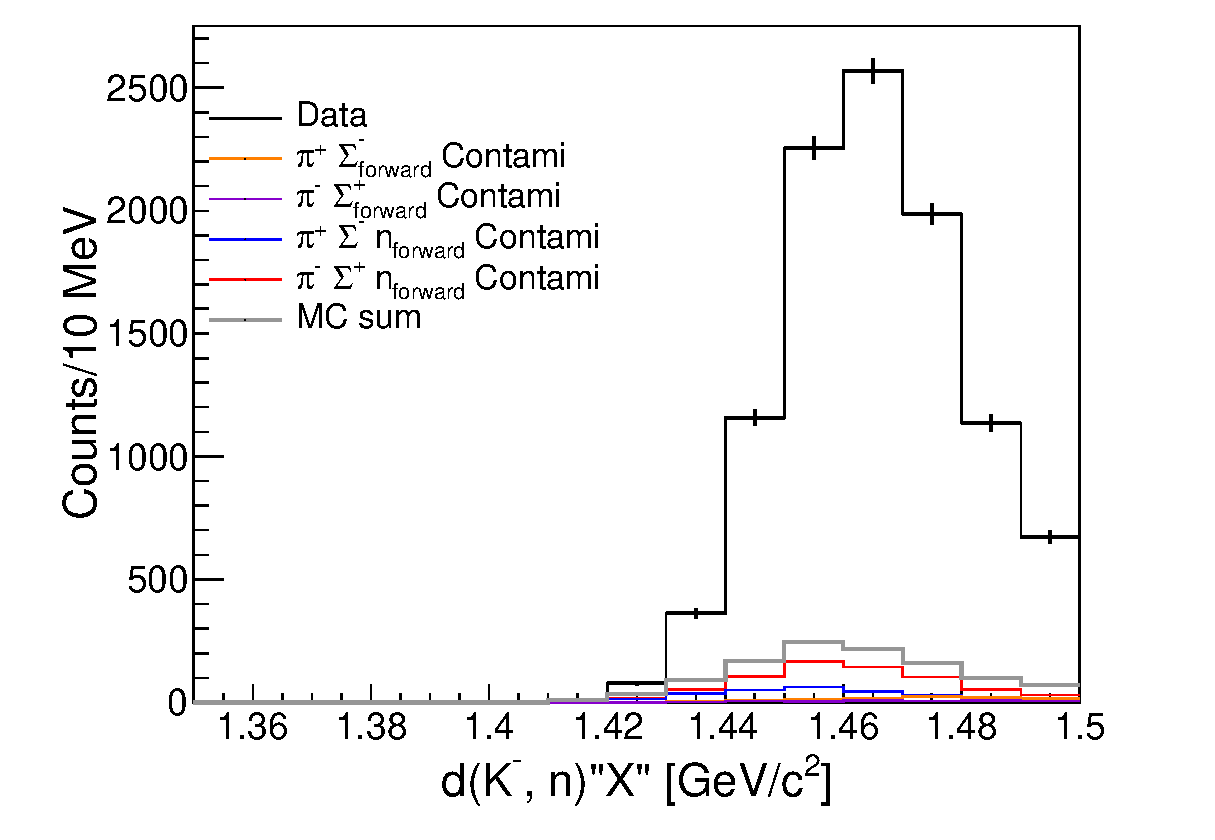
\includegraphics[width=7cm]{../pic/Run78/QE/KN_MM_wK0_tag.eps}
    \end{minipage}
    \begin{minipage}{0.4\hsize}
      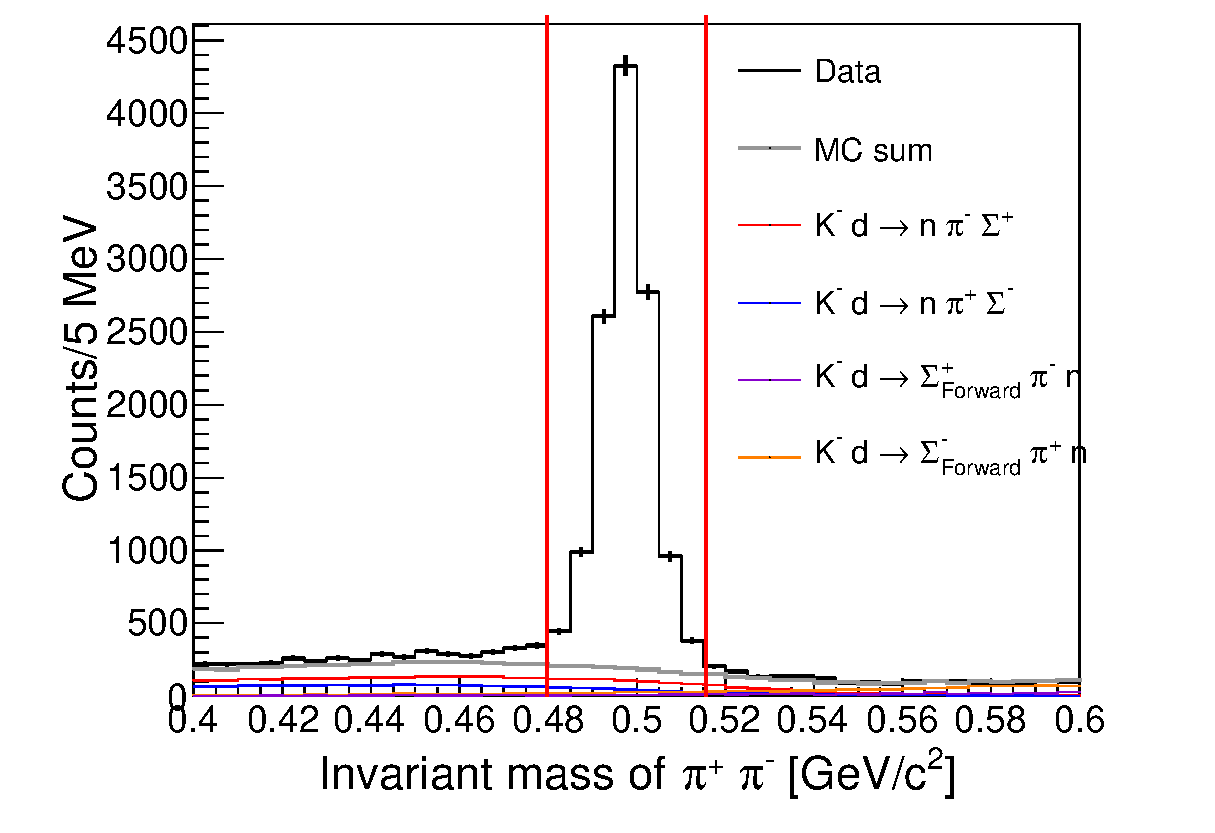
\includegraphics[width=4cm]{../pic/Run78/QE/IM_pipi.eps}
    \end{minipage}
  \end{tabular}
  \caption{
    Right figure shows $K^0$ selection region and estimated background events which is zoom up of left figure of Fig\ref{fig:IM_fit}.
    Red lines indicate selection region.
    left figure shows $d(K^-, n)"n K^0"$ spectra with esmated backgrounds by MC template.
  }
  \label{fig:KN_MM_K0}
\end{figure}
  
$K^0$ identified events is the most strongly candidate to search 1-step reaction of $\bar{K}N$, although the reaction can not measured below the $\bar{K}N$ threshold.
Because $d(K^-, n)"\pi^{\mp}\Sigma^{\pm}"$ reactions is difficulty to reject, each background can be estimated like Fig\ref{fig:IM_fit}.
Fig\cite{fig:KM_MM_K0} indicates $d(K^-, n)"n K^0"$ missing spectrum with estimated backgrounds by template fitting Sec.\ref{sec:temp_fit} (left figure) and
$K^0$ selection gate which is same right figure of Fig\ref{fig:IM_fit} (right figure) without spectra estimated by the Monte Carlo.
In this reaction, $d(K^-, n)$  was rised from the $\bar{K}N$ threshold due to fermi motion of spectator.
The acceptance of this reaction was defined by the $K^0$ kinematics which was detected by the CDS and reconstructed.
So, we estimated the acceptance as function of $K^0$'s $\cos\theta$ and momentum.
We simulate $K^-d\rightarrow K^0 n n$ event with flat mass distribution of $n K^0$ for statistics near the threshold.
Another neutron was scattered forward angle and this neutron was detected by the NC.
The acceptance was estimated by this simulation as Fig\ref{fig:K0_acc}.
$d(K^-, n)"K^0 n"$ spectrum was corrected the acceptance event by event using this 2 dimensional acceptance.
We obtain acceptance corrected spectra as shown in Fig\ref{fig:KN_MM_K0_corr}.
We simultaneously obtain background which was estimated by the Monte Calro simulation to adopt same procedure to background process.
Fig\ref{fig:K0_cos_mom} represents scatter plot of angle and momentum of $K^0$ using data and background process.
Data distribution concentrate to backward and $0.2 GeV$ region which had low acceptance.
On the other hand, background process widly distribute.
By this reson, signal was enhanced by the acceptance correction.
We obtain the cross section of $d(K^-, n)"n K^0"$ to subtrat background and adopt conversion factor of summrized Table\ref{tab:KN_scale} which was shown in Fig\ref{fig:K0_CS}

\begin{figure}[htbp]
  \centering
  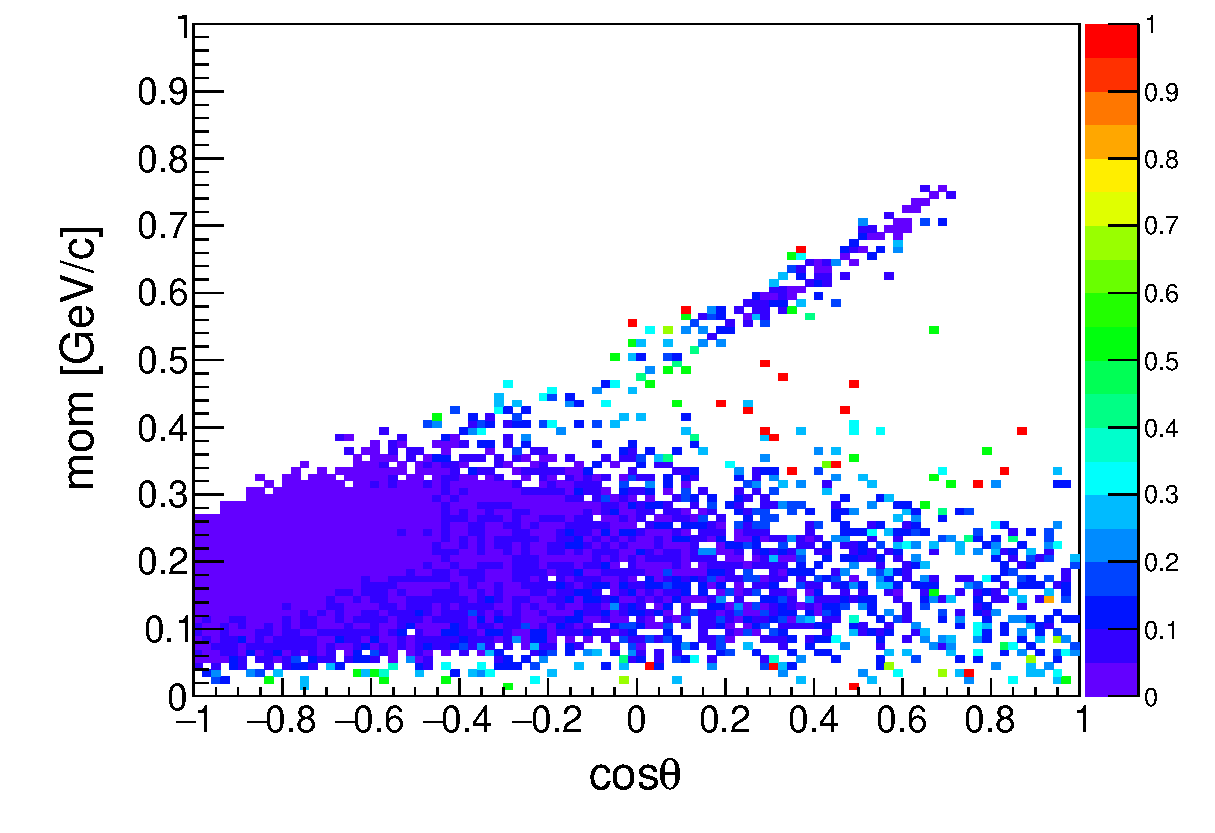
\includegraphics[width=7cm]{../pic/Run78/QE/K0_cos_mom_acc.eps}
  \caption{
    This figure shows the acceptance of the $K^-d\rightarrow K^0 n n$ reaction which was estimated by the Monte Calro simulation.
  }
  \label{fig:K0_acc}
\end{figure}

\begin{figure}[htbp]
  \centering
  \begin{tabular}{cc}
    \begin{minipage}{0.5\hsize}
      \includegraphics[width=7cm]{../pic/Run78/QE/K0_cos_mom_data.eps}
    \end{minipage}

    \begin{minipage}{0.5\hsize}
      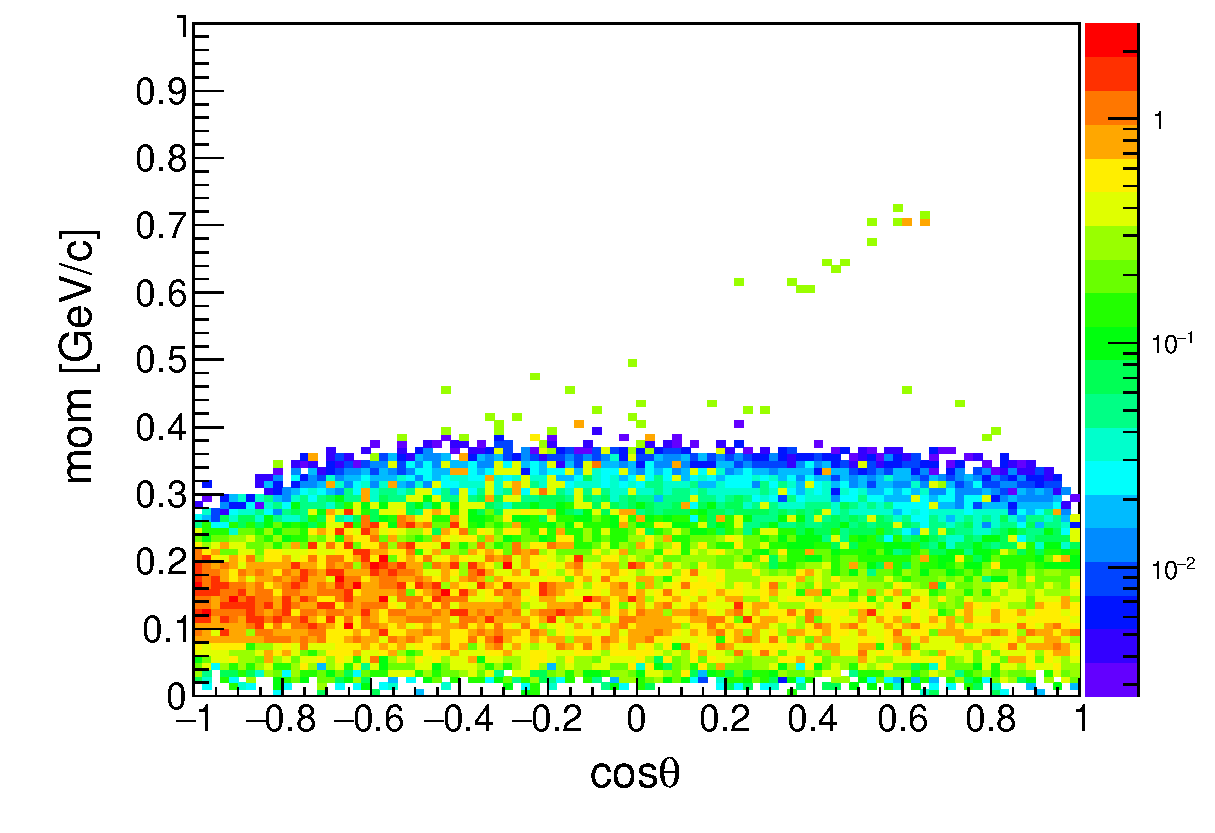
\includegraphics[width=7cm]{../pic/Run78/QE/K0_cos_mom_BG.eps}
    \end{minipage}
  \end{tabular}
  \caption{
    These figure shows about $K^0$ emit angle and momentum in the experimental frame.
    Left figure shows about data and right figure shows background estimated by the Monte Calro.
  }
  \label{fig:K0_cos_mom}
\end{figure}

\begin{figure}[htbp]
  \centering
  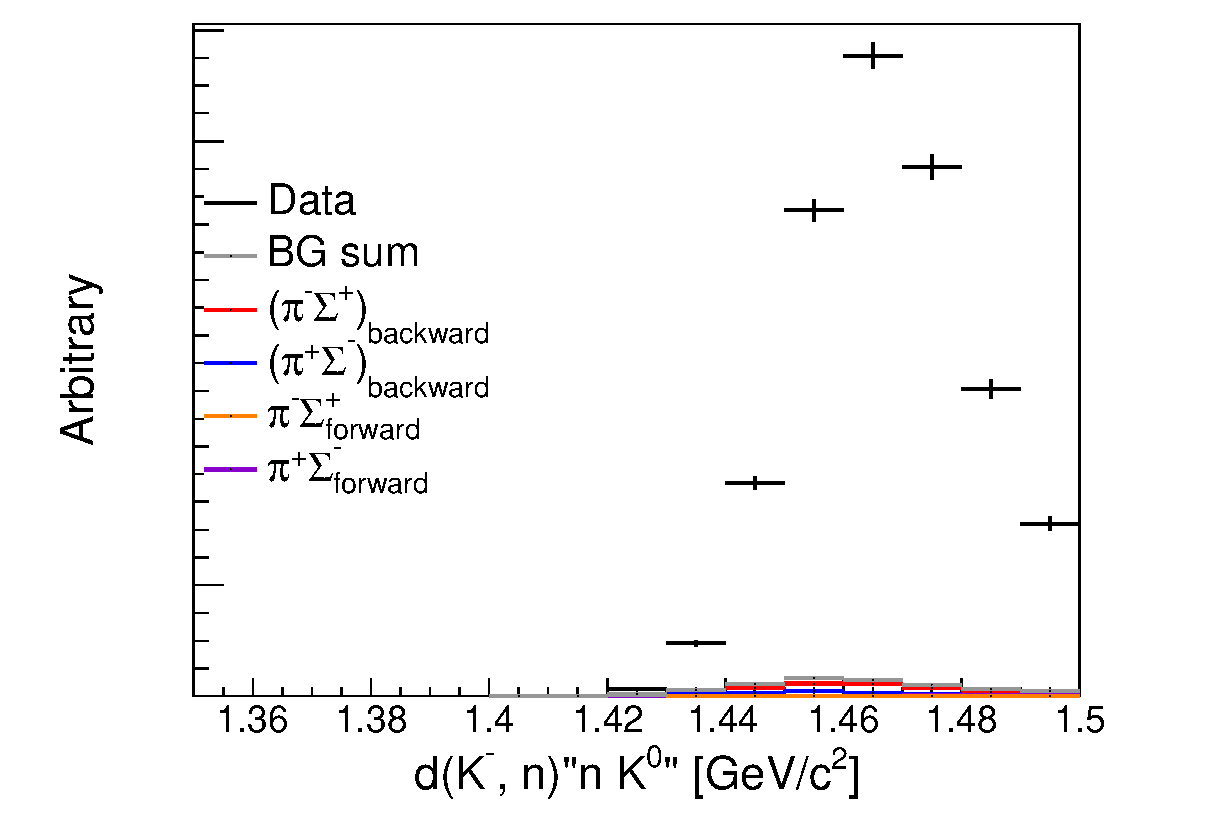
\includegraphics[width=8cm]{../pic/Run78/QE/K0_spec_wBG.eps}
  \caption{
    This figure shows acceptance corrected spectrum of the $d(K^-, n)"n K^0"$.
    Black line indicates data and color plots indicate the background reproduced by the Monte Calro simulation.
  }
  \label{figKN_MM_K0_corr}
\end{figure}
These distribution of data was shown in Fig\ref{fig:K0_cos_mom}.

\begin{figure}[htbp]
  \centering
  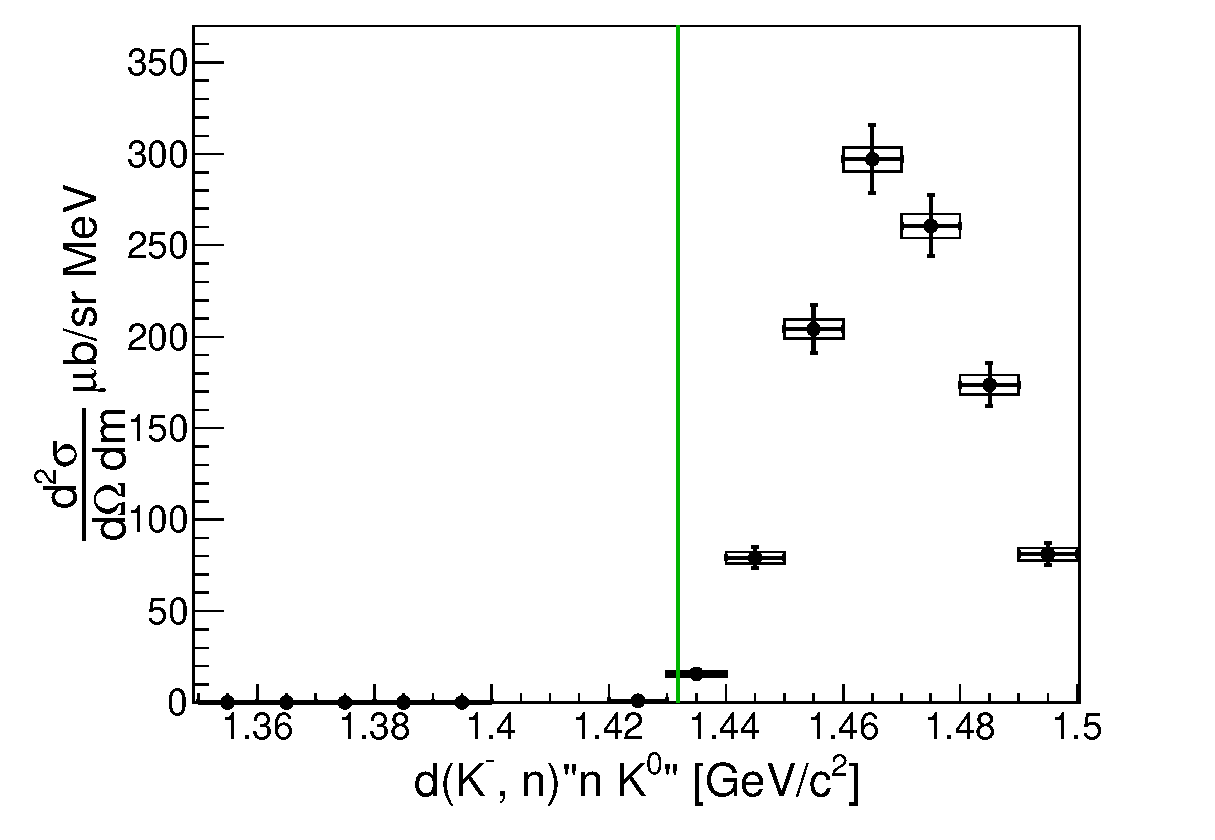
\includegraphics[width=12cm]{../pic/Run78/QE/K0_CS.eps}
  \caption{
    This figure shows the cross section of the $d(K^-, n)"n K^0"$.
    Box indicates statisical errors and error bar indicates errors convolved conversion factors which summrized at Table\ref{tab:KN_scale}
  }
  \label{fig:K0_CS}
\end{figure}

